% Options for packages loaded elsewhere
\PassOptionsToPackage{unicode}{hyperref}
\PassOptionsToPackage{hyphens}{url}
%
\documentclass[
  letterpaper,
]{book}

\usepackage{amsmath,amssymb}
\usepackage{iftex}
\ifPDFTeX
  \usepackage[T1]{fontenc}
  \usepackage[utf8]{inputenc}
  \usepackage{textcomp} % provide euro and other symbols
\else % if luatex or xetex
  \usepackage{unicode-math}
  \defaultfontfeatures{Scale=MatchLowercase}
  \defaultfontfeatures[\rmfamily]{Ligatures=TeX,Scale=1}
\fi
\usepackage{lmodern}
\ifPDFTeX\else  
    % xetex/luatex font selection
\fi
% Use upquote if available, for straight quotes in verbatim environments
\IfFileExists{upquote.sty}{\usepackage{upquote}}{}
\IfFileExists{microtype.sty}{% use microtype if available
  \usepackage[]{microtype}
  \UseMicrotypeSet[protrusion]{basicmath} % disable protrusion for tt fonts
}{}
\makeatletter
\@ifundefined{KOMAClassName}{% if non-KOMA class
  \IfFileExists{parskip.sty}{%
    \usepackage{parskip}
  }{% else
    \setlength{\parindent}{0pt}
    \setlength{\parskip}{6pt plus 2pt minus 1pt}}
}{% if KOMA class
  \KOMAoptions{parskip=half}}
\makeatother
\usepackage{xcolor}
\setlength{\emergencystretch}{3em} % prevent overfull lines
\setcounter{secnumdepth}{5}
% Make \paragraph and \subparagraph free-standing
\ifx\paragraph\undefined\else
  \let\oldparagraph\paragraph
  \renewcommand{\paragraph}[1]{\oldparagraph{#1}\mbox{}}
\fi
\ifx\subparagraph\undefined\else
  \let\oldsubparagraph\subparagraph
  \renewcommand{\subparagraph}[1]{\oldsubparagraph{#1}\mbox{}}
\fi

\usepackage{color}
\usepackage{fancyvrb}
\newcommand{\VerbBar}{|}
\newcommand{\VERB}{\Verb[commandchars=\\\{\}]}
\DefineVerbatimEnvironment{Highlighting}{Verbatim}{commandchars=\\\{\}}
% Add ',fontsize=\small' for more characters per line
\usepackage{framed}
\definecolor{shadecolor}{RGB}{241,243,245}
\newenvironment{Shaded}{\begin{snugshade}}{\end{snugshade}}
\newcommand{\AlertTok}[1]{\textcolor[rgb]{0.68,0.00,0.00}{#1}}
\newcommand{\AnnotationTok}[1]{\textcolor[rgb]{0.37,0.37,0.37}{#1}}
\newcommand{\AttributeTok}[1]{\textcolor[rgb]{0.40,0.45,0.13}{#1}}
\newcommand{\BaseNTok}[1]{\textcolor[rgb]{0.68,0.00,0.00}{#1}}
\newcommand{\BuiltInTok}[1]{\textcolor[rgb]{0.00,0.23,0.31}{#1}}
\newcommand{\CharTok}[1]{\textcolor[rgb]{0.13,0.47,0.30}{#1}}
\newcommand{\CommentTok}[1]{\textcolor[rgb]{0.37,0.37,0.37}{#1}}
\newcommand{\CommentVarTok}[1]{\textcolor[rgb]{0.37,0.37,0.37}{\textit{#1}}}
\newcommand{\ConstantTok}[1]{\textcolor[rgb]{0.56,0.35,0.01}{#1}}
\newcommand{\ControlFlowTok}[1]{\textcolor[rgb]{0.00,0.23,0.31}{#1}}
\newcommand{\DataTypeTok}[1]{\textcolor[rgb]{0.68,0.00,0.00}{#1}}
\newcommand{\DecValTok}[1]{\textcolor[rgb]{0.68,0.00,0.00}{#1}}
\newcommand{\DocumentationTok}[1]{\textcolor[rgb]{0.37,0.37,0.37}{\textit{#1}}}
\newcommand{\ErrorTok}[1]{\textcolor[rgb]{0.68,0.00,0.00}{#1}}
\newcommand{\ExtensionTok}[1]{\textcolor[rgb]{0.00,0.23,0.31}{#1}}
\newcommand{\FloatTok}[1]{\textcolor[rgb]{0.68,0.00,0.00}{#1}}
\newcommand{\FunctionTok}[1]{\textcolor[rgb]{0.28,0.35,0.67}{#1}}
\newcommand{\ImportTok}[1]{\textcolor[rgb]{0.00,0.46,0.62}{#1}}
\newcommand{\InformationTok}[1]{\textcolor[rgb]{0.37,0.37,0.37}{#1}}
\newcommand{\KeywordTok}[1]{\textcolor[rgb]{0.00,0.23,0.31}{#1}}
\newcommand{\NormalTok}[1]{\textcolor[rgb]{0.00,0.23,0.31}{#1}}
\newcommand{\OperatorTok}[1]{\textcolor[rgb]{0.37,0.37,0.37}{#1}}
\newcommand{\OtherTok}[1]{\textcolor[rgb]{0.00,0.23,0.31}{#1}}
\newcommand{\PreprocessorTok}[1]{\textcolor[rgb]{0.68,0.00,0.00}{#1}}
\newcommand{\RegionMarkerTok}[1]{\textcolor[rgb]{0.00,0.23,0.31}{#1}}
\newcommand{\SpecialCharTok}[1]{\textcolor[rgb]{0.37,0.37,0.37}{#1}}
\newcommand{\SpecialStringTok}[1]{\textcolor[rgb]{0.13,0.47,0.30}{#1}}
\newcommand{\StringTok}[1]{\textcolor[rgb]{0.13,0.47,0.30}{#1}}
\newcommand{\VariableTok}[1]{\textcolor[rgb]{0.07,0.07,0.07}{#1}}
\newcommand{\VerbatimStringTok}[1]{\textcolor[rgb]{0.13,0.47,0.30}{#1}}
\newcommand{\WarningTok}[1]{\textcolor[rgb]{0.37,0.37,0.37}{\textit{#1}}}

\providecommand{\tightlist}{%
  \setlength{\itemsep}{0pt}\setlength{\parskip}{0pt}}\usepackage{longtable,booktabs,array}
\usepackage{calc} % for calculating minipage widths
% Correct order of tables after \paragraph or \subparagraph
\usepackage{etoolbox}
\makeatletter
\patchcmd\longtable{\par}{\if@noskipsec\mbox{}\fi\par}{}{}
\makeatother
% Allow footnotes in longtable head/foot
\IfFileExists{footnotehyper.sty}{\usepackage{footnotehyper}}{\usepackage{footnote}}
\makesavenoteenv{longtable}
\usepackage{graphicx}
\makeatletter
\def\maxwidth{\ifdim\Gin@nat@width>\linewidth\linewidth\else\Gin@nat@width\fi}
\def\maxheight{\ifdim\Gin@nat@height>\textheight\textheight\else\Gin@nat@height\fi}
\makeatother
% Scale images if necessary, so that they will not overflow the page
% margins by default, and it is still possible to overwrite the defaults
% using explicit options in \includegraphics[width, height, ...]{}
\setkeys{Gin}{width=\maxwidth,height=\maxheight,keepaspectratio}
% Set default figure placement to htbp
\makeatletter
\def\fps@figure{htbp}
\makeatother

\makeatletter
\@ifpackageloaded{bookmark}{}{\usepackage{bookmark}}
\makeatother
\makeatletter
\@ifpackageloaded{caption}{}{\usepackage{caption}}
\AtBeginDocument{%
\ifdefined\contentsname
  \renewcommand*\contentsname{Table of contents}
\else
  \newcommand\contentsname{Table of contents}
\fi
\ifdefined\listfigurename
  \renewcommand*\listfigurename{List of Figures}
\else
  \newcommand\listfigurename{List of Figures}
\fi
\ifdefined\listtablename
  \renewcommand*\listtablename{List of Tables}
\else
  \newcommand\listtablename{List of Tables}
\fi
\ifdefined\figurename
  \renewcommand*\figurename{Figure}
\else
  \newcommand\figurename{Figure}
\fi
\ifdefined\tablename
  \renewcommand*\tablename{Table}
\else
  \newcommand\tablename{Table}
\fi
}
\@ifpackageloaded{float}{}{\usepackage{float}}
\floatstyle{ruled}
\@ifundefined{c@chapter}{\newfloat{codelisting}{h}{lop}}{\newfloat{codelisting}{h}{lop}[chapter]}
\floatname{codelisting}{Listing}
\newcommand*\listoflistings{\listof{codelisting}{List of Listings}}
\makeatother
\makeatletter
\makeatother
\makeatletter
\@ifpackageloaded{caption}{}{\usepackage{caption}}
\@ifpackageloaded{subcaption}{}{\usepackage{subcaption}}
\makeatother
\ifLuaTeX
  \usepackage{selnolig}  % disable illegal ligatures
\fi
\usepackage[]{natbib}
\bibliographystyle{plainnat}
\usepackage{bookmark}

\IfFileExists{xurl.sty}{\usepackage{xurl}}{} % add URL line breaks if available
\urlstyle{same} % disable monospaced font for URLs
\hypersetup{
  pdftitle={Cast Iron Garden: Plants for Scared People in Central Oklahoma},
  pdfauthor={C.M. Curry and P.M. Cimprich},
  hidelinks,
  pdfcreator={LaTeX via pandoc}}

\title{Cast Iron Garden: Plants for Scared People in Central Oklahoma}
\author{C.M. Curry and P.M. Cimprich}
\date{2024-06-23}

\begin{document}
\frontmatter
\maketitle

\renewcommand*\contentsname{Table of contents}
{
\setcounter{tocdepth}{2}
\tableofcontents
}
\mainmatter
\bookmarksetup{startatroot}

\chapter{What's the deal with native
plants?}\label{whats-the-deal-with-native-plants}

\begin{itemize}
\tightlist
\item
  Help save the world
\item
  Save money
\item
\end{itemize}

\bookmarksetup{startatroot}

\chapter{The really really short version}\label{intro}

\section{Stop killing things}\label{stop-killing-things}

Stop killing insects and plants. If you have plants breaking your
driveway cracks, pour boiling water on it. We'll get to
roundup/bermudagrass/poison ivy in a bit, but for now, just stop until
you know what you are doing.

\section{Stop doing so much unnecessary
work}\label{stop-doing-so-much-unnecessary-work}

Leave the leaves. Leave the twigs. Leave stuff where it falls unless
it's a tripping hazard.

\section{Stop watering stuff that's not in
pots}\label{stop-watering-stuff-thats-not-in-pots}

Save time, save money, save water.

\section{Add in new things between October and April. (NOT IN THE
SUMMER)}\label{add-in-new-things-between-october-and-april.-not-in-the-summer}

Plants are easy if you put them in the right spot, and it's okay if some
die. This book covers a very small area, so I can tell you almost
exactly what's going to work at some place in your yard. But, it's still
okay if some plants die. That's how gardening works. We do our best and
keep going.

Okay, first determine where you are and what kind of soil you have.
-Soil types in Norman area and pictures of them wet and dry and
crumbliness

Almost anywhere in Morman that's sunny and not touching standing water:
- Maximilian sunflower

Shady: - White avens - Lyre Leaf sage - Inland Sea Oats

If you have the red soil and live on the ``north'' (loosely north) side
of town, these are your keystone plants:

If you have the sandy soil and elsewhere in town, plant these:

You can label chapter and section titles using \texttt{\{\#label\}}
after them, e.g., we can reference Chapter @ref(intro). If you do not
manually label them, there will be automatic labels anyway, e.g.,
Chapter @ref(methods).

Figures and tables with captions will be placed in \texttt{figure} and
\texttt{table} environments, respectively.

\begin{Shaded}
\begin{Highlighting}[]
\FunctionTok{par}\NormalTok{(}\AttributeTok{mar =} \FunctionTok{c}\NormalTok{(}\DecValTok{4}\NormalTok{, }\DecValTok{4}\NormalTok{, .}\DecValTok{1}\NormalTok{, .}\DecValTok{1}\NormalTok{))}
\FunctionTok{plot}\NormalTok{(pressure, }\AttributeTok{type =} \StringTok{\textquotesingle{}b\textquotesingle{}}\NormalTok{, }\AttributeTok{pch =} \DecValTok{19}\NormalTok{)}
\end{Highlighting}
\end{Shaded}

\begin{figure}[H]

{\centering 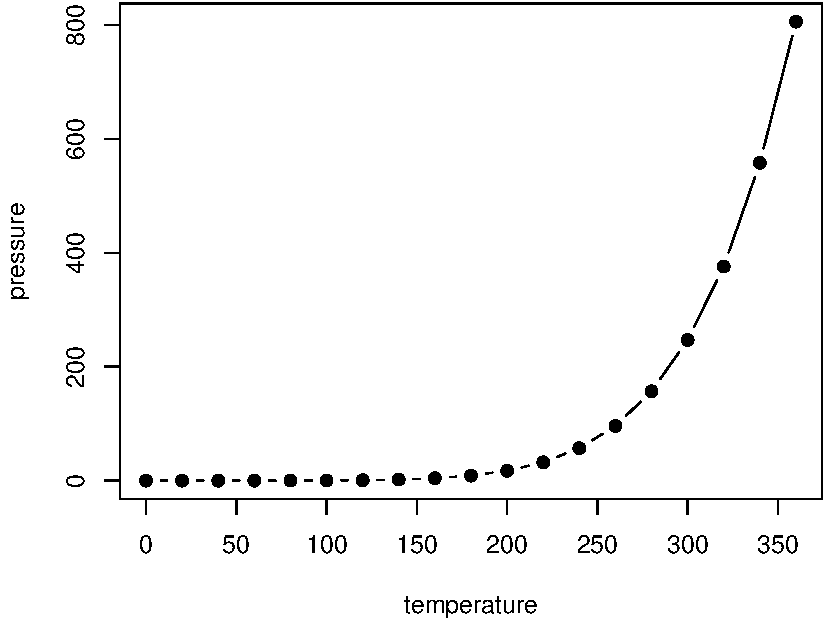
\includegraphics[width=0.8\textwidth,height=\textheight]{01-the_really_really_short_version_files/figure-pdf/nice-fig-1.pdf}

}

\caption{Here is a nice figure!}

\end{figure}%

Reference a figure by its code chunk label with the \texttt{fig:}
prefix, e.g., see Figure @ref(fig:nice-fig). Similarly, you can
reference tables generated from \texttt{knitr::kable()}, e.g., see Table
@ref(tab:nice-tab).

\begin{Shaded}
\begin{Highlighting}[]
\NormalTok{knitr}\SpecialCharTok{::}\FunctionTok{kable}\NormalTok{(}
  \FunctionTok{head}\NormalTok{(iris, }\DecValTok{20}\NormalTok{), }\AttributeTok{caption =} \StringTok{\textquotesingle{}Here is a nice table!\textquotesingle{}}\NormalTok{,}
  \AttributeTok{booktabs =} \ConstantTok{TRUE}
\NormalTok{)}
\end{Highlighting}
\end{Shaded}

\begin{longtable}[]{@{}rrrrl@{}}
\caption{Here is a nice table!}\tabularnewline
\toprule\noalign{}
Sepal.Length & Sepal.Width & Petal.Length & Petal.Width & Species \\
\midrule\noalign{}
\endfirsthead
\toprule\noalign{}
Sepal.Length & Sepal.Width & Petal.Length & Petal.Width & Species \\
\midrule\noalign{}
\endhead
\bottomrule\noalign{}
\endlastfoot
5.1 & 3.5 & 1.4 & 0.2 & setosa \\
4.9 & 3.0 & 1.4 & 0.2 & setosa \\
4.7 & 3.2 & 1.3 & 0.2 & setosa \\
4.6 & 3.1 & 1.5 & 0.2 & setosa \\
5.0 & 3.6 & 1.4 & 0.2 & setosa \\
5.4 & 3.9 & 1.7 & 0.4 & setosa \\
4.6 & 3.4 & 1.4 & 0.3 & setosa \\
5.0 & 3.4 & 1.5 & 0.2 & setosa \\
4.4 & 2.9 & 1.4 & 0.2 & setosa \\
4.9 & 3.1 & 1.5 & 0.1 & setosa \\
5.4 & 3.7 & 1.5 & 0.2 & setosa \\
4.8 & 3.4 & 1.6 & 0.2 & setosa \\
4.8 & 3.0 & 1.4 & 0.1 & setosa \\
4.3 & 3.0 & 1.1 & 0.1 & setosa \\
5.8 & 4.0 & 1.2 & 0.2 & setosa \\
5.7 & 4.4 & 1.5 & 0.4 & setosa \\
5.4 & 3.9 & 1.3 & 0.4 & setosa \\
5.1 & 3.5 & 1.4 & 0.3 & setosa \\
5.7 & 3.8 & 1.7 & 0.3 & setosa \\
5.1 & 3.8 & 1.5 & 0.3 & setosa \\
\end{longtable}

You can write citations, too. For example, we are using the
\textbf{bookdown} package \citep{R-bookdown} in this sample book, which
was built on top of R Markdown and \textbf{knitr} \citep{xie2015}.

\bookmarksetup{startatroot}

\chapter{From the ground up (aka soil, dirt, earth,
etc)}\label{from-the-ground-up-aka-soil-dirt-earth-etc}

Let's call it soil. ``Dirt is what you sweep up'' is another ``all my
weeds are wildflowers''. (who said the dirt vs soil thing?)

Map of Norman with geology maps

Pictures of red clay, sandy loam, sand, and black clay wet and dry

Some plants like some soil. Some like others. We'll tell you which are
which based on what we have tested and read.

\bookmarksetup{startatroot}

\chapter{Reduce, reuse, revegetate}\label{reduce-reuse-revegetate}

Lawn clippings as mulch, compost Lawn post from blog here

\bookmarksetup{startatroot}

\chapter{What about trees?}\label{what-about-trees}

Tree post. What about trees?

\bookmarksetup{startatroot}

\chapter{Garden Calendar}\label{garden-calendar}

-Calendar of seasons and what to do when

\bookmarksetup{startatroot}

\chapter{Species Accounts
Model/Example}\label{species-accounts-modelexample}

-Which plants look dead in the winter but will come back -Is the plant
movable and when is best and how -Species accounts with pictures of all
stages and seeds -How and when can it be pruned -What shape if left
alone? what shape in a group? -What size of containers can it be grown
in? -foot/dog traffic -``agreeableness rating'' a la diboll/cox/voigt
-Observed and published lifespans

Links to all sources (bonap, ladybird center, dave's garden, hostplant
database archive, which books have more info)

Where can purchase (maybe??)

\bookmarksetup{startatroot}

\chapter*{References}\label{references}
\addcontentsline{toc}{chapter}{References}

\markboth{References}{References}

\texttt{r\ if\ (knitr:::is\_html\_output())\ \textquotesingle{}\ \textquotesingle{}}


\backmatter
  \bibliography{references.bib,packages.bib}


\end{document}
